\section{Implementation}

A part of this thesis work was about implementing the new blind rotation algorithm. I chose to start from the open-source FHE library \texttt{OpenFHE} and then add support for the XZDDF blind rotation algorithm to it. In this way, others can hopefully make use of the implementation as well. The implementation is available at
\begin{center}
\url{https://github.com/SL2000s/masters_thesis_xzddf}
\end{center}

The core of \texttt{OpenFHE} consists of two different directories: \texttt{binfhe/} and \texttt{pke/}. The first one only handles fully homomorphic encryption for binary messages and Boolean operations, while the second increases the message space and the number of functions that can be evaluated. Since there was a problem with the original XZDDF algorithm, and the solution suggested in Chapter \ref{sec:xzddf_corr} just works for the Boolean operations, the support for XZDDF was just added to the \texttt{binfhe/} directory.

One thing to note about the implementation is that the paper by Xiang et al. \cite{cite:fast_bootstrap_crypto23} assumes that the $\operatorname{LWE}$ encryption is on the form 
$$c = \operatorname{LWE}_{q,\mathbf{s}}(m) = \left(\mathbf{a}, b = \langle \mathbf{a}, \mathbf{s} \rangle - \operatorname{noised}(m)\right),$$
so that the decryption algorithm becomes 
$$\operatorname{Dec}(c) = \langle \mathbf{a}, \mathbf{s} \rangle - b,$$
but the $\operatorname{LWE}$ encryption in \texttt{OpenFHE} is implemented as
$$c = \operatorname{LWE}_{q,\mathbf{s}}(m) = \left(\mathbf{a}, b = \langle \mathbf{a}, \mathbf{s} \rangle + m \cdot \frac{q}{t} + e\right),$$
with the decryption algorithm
$$\operatorname{Dec}(c) = b - \langle \mathbf{a}, \mathbf{s} \rangle.$$

%This was easily solved by setting $\Delta = -\frac{Q}{8}$ instead of $\Delta = \frac{Q}{8}$, and then modifying equation (\ref{eq:noised_m}) to
This was easily solved by modifying (\ref{eq:noised_m}) to
$$\operatorname{noised}(m) = \operatorname{coeff}_0 \left(r(X^{\frac{2N}{q}}) \cdot X^{\frac{2N}{q}b} X^{\sum_{i=0}^{n-1}-w_is_i} X^{\sum_{i=0}^{n-1}s_i}\right),$$
where $w_i=\frac{2N}{q}a_i+1$ as before.

\section{Testing Methods}\label{subsec:methods}

After having implemented the algorithm, the efficiency of it was tested. The efficiency tests can be found at the following link.

\begin{center}
\url{https://github.com/SL2000s/masters_thesis_xzddf/tree/main/benchmark}
\end{center}

Using Regev LWE encryption as the first-layer encryption algorithm, the tests timed a few different actions a user potentially would like to do when using FHE encryption. We divide the tests into two categories: simple tests (Table \ref{tab:simple_tests}), and batch tests (Table \ref{tab:batch_tests}).

\begin{table}[ht]
\centering
\caption{Description of some simple tests that were performed.}
\begin{tabular}{cl}
\toprule
\textbf{Test} & \textbf{Description} \\
\midrule
\text{S1:} & Generate a bootstrapping key. \\
\text{S2:} & Perform a single bootstrapping. \\
\text{S3:} & Perform an OR operation on two ciphertexts \(c_0\) and \(c_1\). \\
\text{S4:} & Perform an AND operation on two ciphertexts \(c_0\) and \(c_1\). \\
\bottomrule
\end{tabular}
\label{tab:simple_tests}
\end{table}

In the batch tests, where a ciphertext $c_1$ was updated $x$ times in a row by the following sequence of homomorphic operations:
$$c_1 \gets \operatorname{NOT}(\operatorname{AND}(c_0, \operatorname{OR}(c_0, c_1))) =: f(c_0,c_1).$$

\begin{table}[ht]
\centering
\caption{Description of the batch tests that were performed.}
\begin{tabular}{cl}
\toprule
\textbf{Test} & \textbf{Description} \\
\midrule
\text{B1:} & Update $c_1$ with the value of $f(c_0,c_1)$ 1 time. \\
\text{B2:} & Update $c_1$ with the value of $f(c_0,c_1)$ 10 times. \\
\text{B3:} & Update $c_1$ with the value of $f(c_0,c_1)$ 100 times. \\
\text{B4:} & Update $c_1$ with the value of $f(c_0,c_1)$ 1000 times. \\
\bottomrule
\end{tabular}
\label{tab:batch_tests}
\end{table}

% \underline{Simple tests:}
% \begin{itemize}
%     \item \textbf{Test 1}: Generating a bootstrapping key.
%     \item \textbf{Test 2}: Performing a single bootstrapping.
%     \item \textbf{Test 3}: Performing an OR operation on two ciphertexts $c_1$ and $c_2$.
%     \item \textbf{Test 4}: Performing an AND operation on two ciphertexts $c_1$ and $c_2$.
% \end{itemize}

% \underline{Batch tests:}
% \begin{itemize}
%     \item \textbf{Test 5}: Performing the following sequence of binary operations 1 times: $$c_2 = \operatorname{NOT}(\operatorname{AND}(c_1, \operatorname{OR}(c_1, c_2))).$$
%     \item \textbf{Test 6}: Performing the following sequence of binary operations 10 times: $$c_2 = \operatorname{NOT}(\operatorname{AND}(c_1, \operatorname{OR}(c_1, c_2))).$$
%     \item \textbf{Test 7}: Performing the following sequence of binary operations 100 times: $$c_2 = \operatorname{NOT}(\operatorname{AND}(c_1, \operatorname{OR}(c_1, c_2))).$$
%     \item \textbf{Test 9}: Performing the following sequence of binary operations 1000 times: $$c_2 = \operatorname{NOT}(\operatorname{AND}(c_1, \operatorname{OR}(c_1, c_2))).$$
% \end{itemize}

% \underline{Old:}
% \begin{itemize}
%     \item \textbf{Test 1}: Generating a bootstrapping key.
%     \item \textbf{Test 2}: Performing an OR operation on two ciphertexts $c_1$ and $c_2$.
%     \item \textbf{Test 3}: Performing an AND operation on two ciphertexts $c_1$ and $c_2$.
%     \item \textbf{Test 4}: Performing the following sequence of binary operations 10 times: $$c_2 = \operatorname{NOT}(\operatorname{AND}(c_1, \operatorname{OR}(c_1, c_2))).$$
%     \item TODO: add batch test
%     \item TODO: add single bootstrapping test
% \end{itemize}

In all tests, the ciphertexts were initially $(c_0, c_1)=(1,0)$. For the simple tests \linebreak S1--S4, and for the batch tests B1--B2, the actions were executed 100 times each, and then the average execution time was computed. For Test B3 and B4, the average execution time was instead computed over 10 tests and 3 tests, respectively, to decrease the total execution time for the test.

All of the blind rotation algorithms AP, GINX, LMKCDEY, and XZDDF were tested with the same setup. Each algorithm was tested with one parameter set corresponding to 128-bit security, and one parameter set corresponding to 192-bit security. Table \ref{tab:paramsets} shows the parameter values in each parameter set. The key distribution for each parameter set was either ternary, i.e. $\mathcal{U}(\{-1,0,1\})$, or discrete Gaussian with mean 0 and standard deviation 3.19, i.e. $\mathcal{N}_{\mathbb{Z}}(0, 3.19^2)$. For XZDDF, the four optimized parameter sets (P128T, P128G, P192T, and P192G) from Xiang et al. \cite{cite:fast_bootstrap_crypto23} were tested as well.

%The first parameter set corresponded to $\lambda = 128$ bits security, and the second to $\lambda = 192$ bits security. 

\begin{table}[ht]
\centering
\caption{The parameter sets for bootstrapping in \texttt{OpenFHE}. P128T, P128G, P192T, and P192G are designed for XZDDF \cite{cite:fast_bootstrap_crypto23}. STD128L (called STD128\_LMKCDEY in \texttt{OpenFHE}) is designed for LMKCDEY.}
\begin{tabular}{l|cccccccc}
\toprule
\textbf{Set} & \textbf{Dist.} & $n$ & $q$ & $N$ & $Q$ & $B$ & $Q_{\text{ks}}$ & $B_{\text{ks}}$ \\
\midrule
STD128 & Tern. & 503 & 1024 & 1024 & 134215681 & $2^{9}$ & $2^{14}$ & $2^5$ \\
STD128L & Gauss. & 446 & 1024 & 1024 & 268369921 & $2^{10}$ & $2^{13}$ & $2^{5}$ \\
P128T & Tern. & 512 & 1024 & 1024 & 995329 & $2^{4}$ & $2^{14}$ & $2^7$ \\
P128G & Gauss. & 465 & 1024 & 1024 & 995329 & $2^{4}$ & $2^{14}$ & $2^7$ \\
STD192 & Tern. & 805 & 1024 & 2048 & 137438822401 & $2^{13}$ & $2^{15}$ & $2^5$ \\
P192T & Tern. & 1024 & 1024 & 2048 & 44421121 & $2^{9}$ & $2^{19}$ & 28 \\
P192G & Gauss. & 870 & 1024 & 2048 & 44421121 & $2^{9}$ & $2^{17}$ & 28 \\
\bottomrule
\end{tabular}
\label{tab:paramsets}
\end{table}

At last, the tests S3 and S4 were also performed with the original rotation polynomial in the XZDDF paper \cite{cite:fast_bootstrap_crypto23}. This implementation can be found in the branch \texttt{XZDDF\_original} of the \texttt{GitHub} repository.

%The tests were performed on a laptop with the processor "Intel Core i7-6600U CPU @ 2.60GHz × 4".
The tests were conducted on a laptop equipped with an Intel Core i7-6600U CPU running at 2.60GHz (4 cores). To decrease noise in the result caused by background activities as much as possible, all other programs on the computer were shut down before the test, and the internet connection was also turned off.

\section{Results}

The results when doing the simple tests can be seen in Table \ref{tab:efficiency_res}. In Appendix \ref{sec:appendix_figures}, Figure \ref{fig:distr_brkgen1}--\ref{fig:distr_10andornot2} show the distribution of the execution times. 

\begin{table}[ht]
\centering
\caption{The execution time for different bootstrapping algorithms and different security levels $\lambda$ (in bits), when performing the four simple tests S1--S4 described in Table \ref{tab:simple_tests}.}
\begin{tabular}{lc|cccc}
\toprule
\textbf{Algorithm} & \textbf{Param.} & \textbf{S1} (ms)  & \textbf{S2} (ms) & \textbf{S3} (ms) & \textbf{S4} (ms) \\
\midrule
AP & STD128 & 10541 & 182 & 175 & 175 \\
GINX & STD128 & 2583 & 153 & 145 & 145 \\
LMKCDEY & STD128L & 2121 & 120 & 132 & 134 \\
XZDDF & STD128 & 2438 & 174 & 184 & 185 \\
XZDDF & P128T & 6386 & 214 & 216 & 216 \\
XZDDF & P128G & 5820 & 194 & 195 & 195 \\
AP & STD192 & 38489 & 651 & 662 & 645 \\
GINX & STD192 & 8546 & 467 & 467 & 468 \\
LMKCDEY & STD192 & 8833 & 493 & 512 & 435 \\
XZDDF & STD192 & 8391 & 626 & 622 & 626 \\
XZDDF & P192T & 11808 & 700 & 699 & 699 \\
XZDDF & P192G & 9989 & 592 & 592 & 592 \\
\bottomrule
\end{tabular}
\label{tab:efficiency_res}
\end{table}

% OLD!
% \begin{table}[ht]
% \centering
% \begin{tabular}{lc|cccc}
% \toprule
% \textbf{Algorithm} & $\lambda$ & \textbf{Test 1}  & \textbf{Test 2}  & \textbf{Test 3}  & \textbf{Test 4}  \\
% %\textbf{rithm} &  & (ms)  & (ms)  & (ms)  & (ms)  \\
% \midrule
% AP & 128 & 10800 ms & 185 ms & 186 ms & 3892 ms \\
%     GINX & 128 & 2940 ms & 162 ms & 151 ms & 3527 ms \\
%     %LMKCDEY & 128 & 2686 ms & 166 ms & 163 ms & 2687 ms \\
%     XZDDF & 128 & 2829 ms & 183 ms & 181 ms & 3575 ms \\
%     AP & 192 & 41361 ms & 711 ms & 859 ms & 14415 ms \\
%     GINX & 192 & 8956 ms & 560 ms & 628 ms & 11280 ms \\
%     %LMKCDEY & 192 & 9088 ms & 470 ms & 461 ms & 9679 ms \\
%     XZDDF & 192 & 8629 ms & 680 ms & 688 ms & 13750 ms \\
%     \bottomrule
% \end{tabular}
% \caption{The execution time for different bootstrapping algorithms and different security levels $\lambda$ (in bits), when performing the four tests described in Section \ref{subsec:methods}.}
% \label{tab:efficiency_res}
% \end{table}

The results when doing the batch tests can be seen in Table \ref{tab:batch_res}. In Appendix \ref{sec:appendix_figures}, Figure \ref{fig:batch1}--\ref{fig:batch2} show log-log plots of the execution times for each bootstrapping algorithm and each parameter set.

\begin{table}[ht]
\centering
\caption{The execution time for different bootstrapping algorithms and different security levels $\lambda$ (in bits), when performing the batch tests B1--B4 described in Table \ref{tab:batch_tests}.}
\begin{tabular}{lc|cccc}
\toprule
\textbf{Algorithm} & \textbf{Param.} & \textbf{B1} (ms)  & \textbf{B2} (ms) & \textbf{B3} (ms) & \textbf{B4} (ms) \\
\midrule
AP & STD128 & 350 & 3476 & 35364 & 355842 \\
GINX & STD128 & 293 & 2898 & 29325 & 315418 \\
LMKCDEY & STD128L & 259 & 2475 & 28362 & 280270 \\
XZDDF & STD128 & 330 & 3687 & 33481 & 331717 \\
XZDDF & P128T & 432 & 4316 & 42416 & 426885 \\
XZDDF & P128G & 392 & 3925 & 38949 & 391517 \\
AP & STD192 & 1146 & 13052 & 115382 & 1213410 \\
GINX & STD192 & 949 & 9417 & 96319 & 1005410 \\
LMKCDEY & STD192 & 854 & 8172 & 86082 & 822024 \\
XZDDF & STD192 & 1254 & 12439 & 114381 & 1163360 \\
XZDDF & P192T & 1397 & 13913 & 139535 & 1387043 \\
XZDDF & P192G & 1183 & 11799 & 117632 & 1175503 \\
\bottomrule
\end{tabular}
\label{tab:batch_res}
\end{table}

Figure \ref{fig:decr_fail} shows an example of a decryption failure when using the original XZDDF algorithm.

\begin{figure}
    \centering
    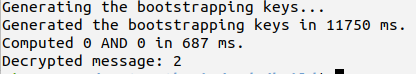
\includegraphics[trim={2 2 5 0},clip,width=0.8\linewidth]{data/figures/failure.png}
    \caption{Decryption failure when using the original rotation polynomial. The AND operation is performed on two zeros, so the result should be 0.}
    \label{fig:decr_fail}
\end{figure}


\section{Discussion}

Looking at Table \ref{tab:efficiency_res}, we see that when using STD128, XZDDF is among the fastest when generating the evaluation key (Test S1), beating all other algorithms except 128-bit secure LMKCDEY. This aligns quite well with the results of Xiang et al. \cite{cite:fast_bootstrap_crypto23}, where XZDDF was faster in all tests. However, theoretically, the key generation should be even faster than in Table \ref{tab:efficiency_res} -- at least twice the speed of LMKCDEY and even faster when compared with AP and GINX.

The measured execution time of 128-bit secure XZDDF might be slower than 128-bit LMKCDEY due to noise since 192-bit XZDDF is faster than 192-bit LMKCDEY, but it might also be slower because \texttt{OpenFHE} has an optimized security parameter set for LMKCDEY when using 128-bit security (STD192L), but not for 192-bit security.

When using the parameter sets P128T, P128G, P192T, and P192G from Xiang et al., designed specifically for XZDDF, we see that the key generation (Test S1) is significantly slower for these than when using STD128. This is probably due to the larger $n$, resulting in a longer vector of values to compute in the evaluation key. However, the performance of the homomorphic operations is better, although still slower than when using STD128 for XZDDF.

Just as the results of Xiang et al. \cite{cite:fast_bootstrap_crypto23}, there seems to be a small efficiency gain when using a Gaussian distribution instead of a uniformly ternary distribution (compare P128T vs. P128G, and P192T vs. P192G in Table \ref{tab:efficiency_res}).

When looking at the results of Test S2--S4 in Table \ref{tab:efficiency_res}, one can first note that the Boolean operations (which include one bootstrapping) take about the same time as just performing a single bootstrapping. This is as expected because bootstrapping is the main bottleneck in FHE. In \texttt{OpenFHE}, Boolean operations involve one addition and one bootstrapping, with the addition being performed basically instantly compared to the bootstrapping.

Next, one can note that the XZDDF implementation does not seem to perform bootstrapping better than GINX and LMKCDEY, and just marginally better than AP. This differs from the results of Xiang et al. \cite{cite:fast_bootstrap_crypto23}, where the XZDDF bootstrapping was more than two times faster than GINX and even faster compared to AP (see e.g. Table 5 in \cite{cite:fast_bootstrap_crypto23}).

One possible explanation for this is that the other implementations have existed for a longer time in \texttt{OpenFHE}, so a lot of good programmers have had time to read the code and optimize it. The XZDDF implementation in this project likely has parts that can be optimized more.

There are two different ways to represent polynomials in the \texttt{OpenFHE} library -- \texttt{Format::COEFFICIENT} and \texttt{Format::EVALUATION}. The first representation is probably what we are used to -- a vector of coefficients -- while the second format is a format that makes polynomial multiplications more efficient. The XZDDF implementation switches polynomials back and forth between these representations a few times. Some switches are necessary, but each switch seems to be significantly inefficient. Therefore, if one aims to optimize the XZDDF implementation further, reducing the number of format switches might be a good starting point.

In Figure \ref{fig:distr_brkgen1}--\ref{fig:distr_10andornot2}, we see that the distributions of the measured execution times usually seem to have a high peak around one value, and then a smaller number of measured times around that peak. There are some exceptions, e.g. 128-bit secure GINX in Figure \ref{fig:distr_and1} that has two peaks, which could be interesting to investigate further, but a possible explanation for these figures is that they arose due to noise, e.g. some background activity on the computer.

In Table \ref{tab:batch_res} and in Figure \ref{fig:batch1}--\ref{fig:batch2}, we see that the execution time of multiple Boolean operations in a row seems to be linear in the number of operations. This is also logical since the part of the \texttt{OpenFHE} library that was used for testing did not support any batching of operations, so the Boolean operations were always followed by a bootstrapping operation.


%This aligns with the results in \cite{cite:fast_bootstrap_crypto23}, although the result there was that XZDDF was about three times faster than AP and two times faster than GINX. However, when doing the bootstrapping itself, the XZDDF implementation seemed to be a bit slower than GINX. Looking at the time complexity of the algorithms (see eg. Table 1 in \cite{cite:fast_bootstrap_crypto23}), this should not be the case. One explanation for this is that the AP and GINX implementations have already existed for a few years in \texttt{OpenFHE}, so a lot of good programmers have had time to read the code and optimize it. The XZDDF implementation in this project probably has parts that can be optimized more.